\documentclass[conference]{IEEEtran}
\IEEEoverridecommandlockouts
\usepackage{cite}
\usepackage{amsmath,amssymb,amsfonts}
\usepackage{algorithmic}
\usepackage{graphicx}
\usepackage{textcomp}
\usepackage{xcolor}
\usepackage{booktabs}
\usepackage{multirow}
\usepackage{url}

\def\BibTeX{{\rm B\kern-.05em{\sc i\kern-.025em b}\kern-.08em
    T\kern-.1667em\lower.7ex\hbox{E}\kern-.125emX}}

\begin{document}

\title{Unsupervised Latent Health State Discovery and Sequential Dynamics in Longitudinal Wearable Physiology: A Methodological Benchmark}

\author{\IEEEauthorblockN{Lokesh S.}
\IEEEauthorblockA{\textit{Department of Computer Science and Engineering} \\
\textit{Wearable Health AI Analytics Group}\\
India \\
slokesh2205@gmail.com}
}

\maketitle

\begin{abstract}
Continuous physiological monitoring via consumer wearable devices offers unprecedented opportunities for personalized longitudinal health tracking. However, modelling wearable physiology is severely complicated by high inter-individual baseline variation, non-stationary daily dynamics, sensor noise, and a lack of continuous clinical diagnostic ground-truth labels. In this paper, we present a causal, leakage-controlled methodological framework for unsupervised latent health state discovery and dynamic sequence modeling from multi-month wearable physiological timelines. Our pipeline transforms raw multi-modal signals into personalized 7-day rolling baseline deviations, composite homeostatic disruption severity scores, and continuous Gaussian Mixture Model (GMM) posterior probability vectors, followed by sequential Hidden Markov Model (HMM) decoding. Evaluating our framework across a longitudinal cohort of 300 user timelines comprising 55,200 daily observations (184 days per user), we demonstrate through 5-fold subject-independent cross-validation across unseen users that personalized baseline deviations significantly improve static cluster separation ($d = 4.6119$, mean Silhouette $0.1940$ vs. $0.1601$ for raw physiology; Wilcoxon $W = 0.0$, $p = 0.0625$, bounded by $N=5$ sample size). We further conduct an empirical degeneracy analysis revealing that continuous Gaussian HMMs trained over low-entropy GMM posterior vectors collapse into single-state absorption (100\% state occupancy), whereas discrete Categorical HMMs successfully capture multi-state temporal transitions across Recovery (22.69\%), Baseline (26.92\%), and Strain (50.39\%) states with a mean run duration of 1.51 days. A surrogate Random Forest model provides SHAP-like feature attributions with 96.5\% classification fidelity to support explainable dashboard visualization.
\end{abstract}

\begin{IEEEkeywords}
Wearable physiological signals, baseline deviations, Gaussian Mixture Model, Hidden Markov Model, unsupervised state discovery, temporal dynamics, empirical benchmark.
\end{IEEEkeywords}

\section{Introduction}
Longitudinal physiological tracking using consumer-grade wearable sensors—such as smartwatches, continuous heart rate monitors, and sleep trackers—has transitioned health monitoring from intermittent clinical visits to continuous free-living observation \cite{b1}. Wearable devices measure key physiological indicators including resting heart rate (RHR), heart rate variability (HRV), blood oxygen saturation ($\text{SpO}_2$), nightly sleep duration, and physical activity levels. These multi-modal signals reflect acute physiological stress, circadian rhythms, physical strain, and homeostatic recovery \cite{b2}.

Despite the rich temporal density of wearable datasets, modeling free-living wearable physiology introduces distinct data science challenges:
\begin{enumerate}
    \item \textbf{Inter-Individual Baseline Heterogeneity}: Baseline physiological values differ substantially between individuals due to age, biological sex, cardiorespiratory fitness, and genetic factors. For instance, a resting heart rate of 75 beats per minute (bpm) may indicate acute cardiovascular strain for an endurance athlete but ideal baseline recovery for a sedentary individual \cite{b3}.
    \item \textbf{Non-Stationary Time Series Dynamics}: Wearable signals exhibit natural diurnal fluctuations, weekly activity patterns, and seasonal drift, making static global thresholds inadequate for detecting meaningful physiological shifts.
    \item \textbf{Absence of Clinical Ground-Truth Labels}: Free-living wearable monitoring lacks continuous clinical diagnostic labels. Unsupervised state discovery methods must therefore identify interpretable, coherent latent health states without supervisory signals \cite{b4}.
    \item \textbf{Data Leakage Pitfalls in Time Series}: Unintended look-ahead bias—such as backward missing value imputation (\texttt{bfill}), non-causal outlier capping over future horizons, or fitting feature scalers across entire cohorts—artificially inflates performance metrics and renders models non-deployable in prospective real-time settings \cite{b5}.
\end{enumerate}

To address these challenges, we propose a causal, leakage-controlled framework that combines personalized baseline deviation encoding, probabilistic density estimation via Gaussian Mixture Models (GMM), and temporal state sequence modeling via Hidden Markov Models (HMM). Our framework isolates static clustering from sequential dynamics, enabling robust state discovery across longitudinal timelines.

The primary contributions of this paper are fourfold:
\begin{itemize}
    \item \textbf{Causal Leakage-Controlled Preprocessing Architecture}: We define a strict causal preprocessing pipeline incorporating forward-only missing value fill, expanding causal Interquartile Range (IQR) outlier capping, a mandatory 7-day baseline warm-up requirement ($\text{min\_periods}=7$), and train-set-only feature scaling.
    \item \textbf{Personalized State Discovery Benchmark}: We conduct a comprehensive empirical evaluation of six baseline methods ($\text{B0}$–$\text{B6}$) and a seven-step component ablation ($\text{A}$–$\text{G}$) on a longitudinal cohort of 300 users (55,200 daily observations over 184 days).
    \item \textbf{Subject-Independent Generalizability Analysis}: Using 5-fold grouped cross-validation across unseen user timelines, we show that personalized baseline deviation features paired with composite severity normalization achieve a standardized effect size of $d = 4.6119$ over raw physiological features. We provide a rigorous statistical discussion on the mathematical boundary of $N=5$ Wilcoxon non-parametric testing ($p = 0.0625 > 0.05$).
    \item \textbf{Empirical HMM Degeneracy Discovery}: We report a critical negative result: continuous Gaussian HMMs trained over low-entropy GMM soft posterior vectors degenerate into a single absorbing state (100\% occupancy in a single state), whereas hard Categorical HMMs maintain active multi-state dynamics across Recovery ($22.69\%$), Baseline ($26.92\%$), and Strain ($50.39\%$).
\end{itemize}

\textit{Non-Clinical Disclosure}: This work presents an algorithmic methodological benchmark for longitudinal wearable analytics using a synthetic longitudinal physiological cohort. It does not provide clinical diagnosis, medical decision support, or clinical trial validation.

\begin{figure}[htbp]
\centerline{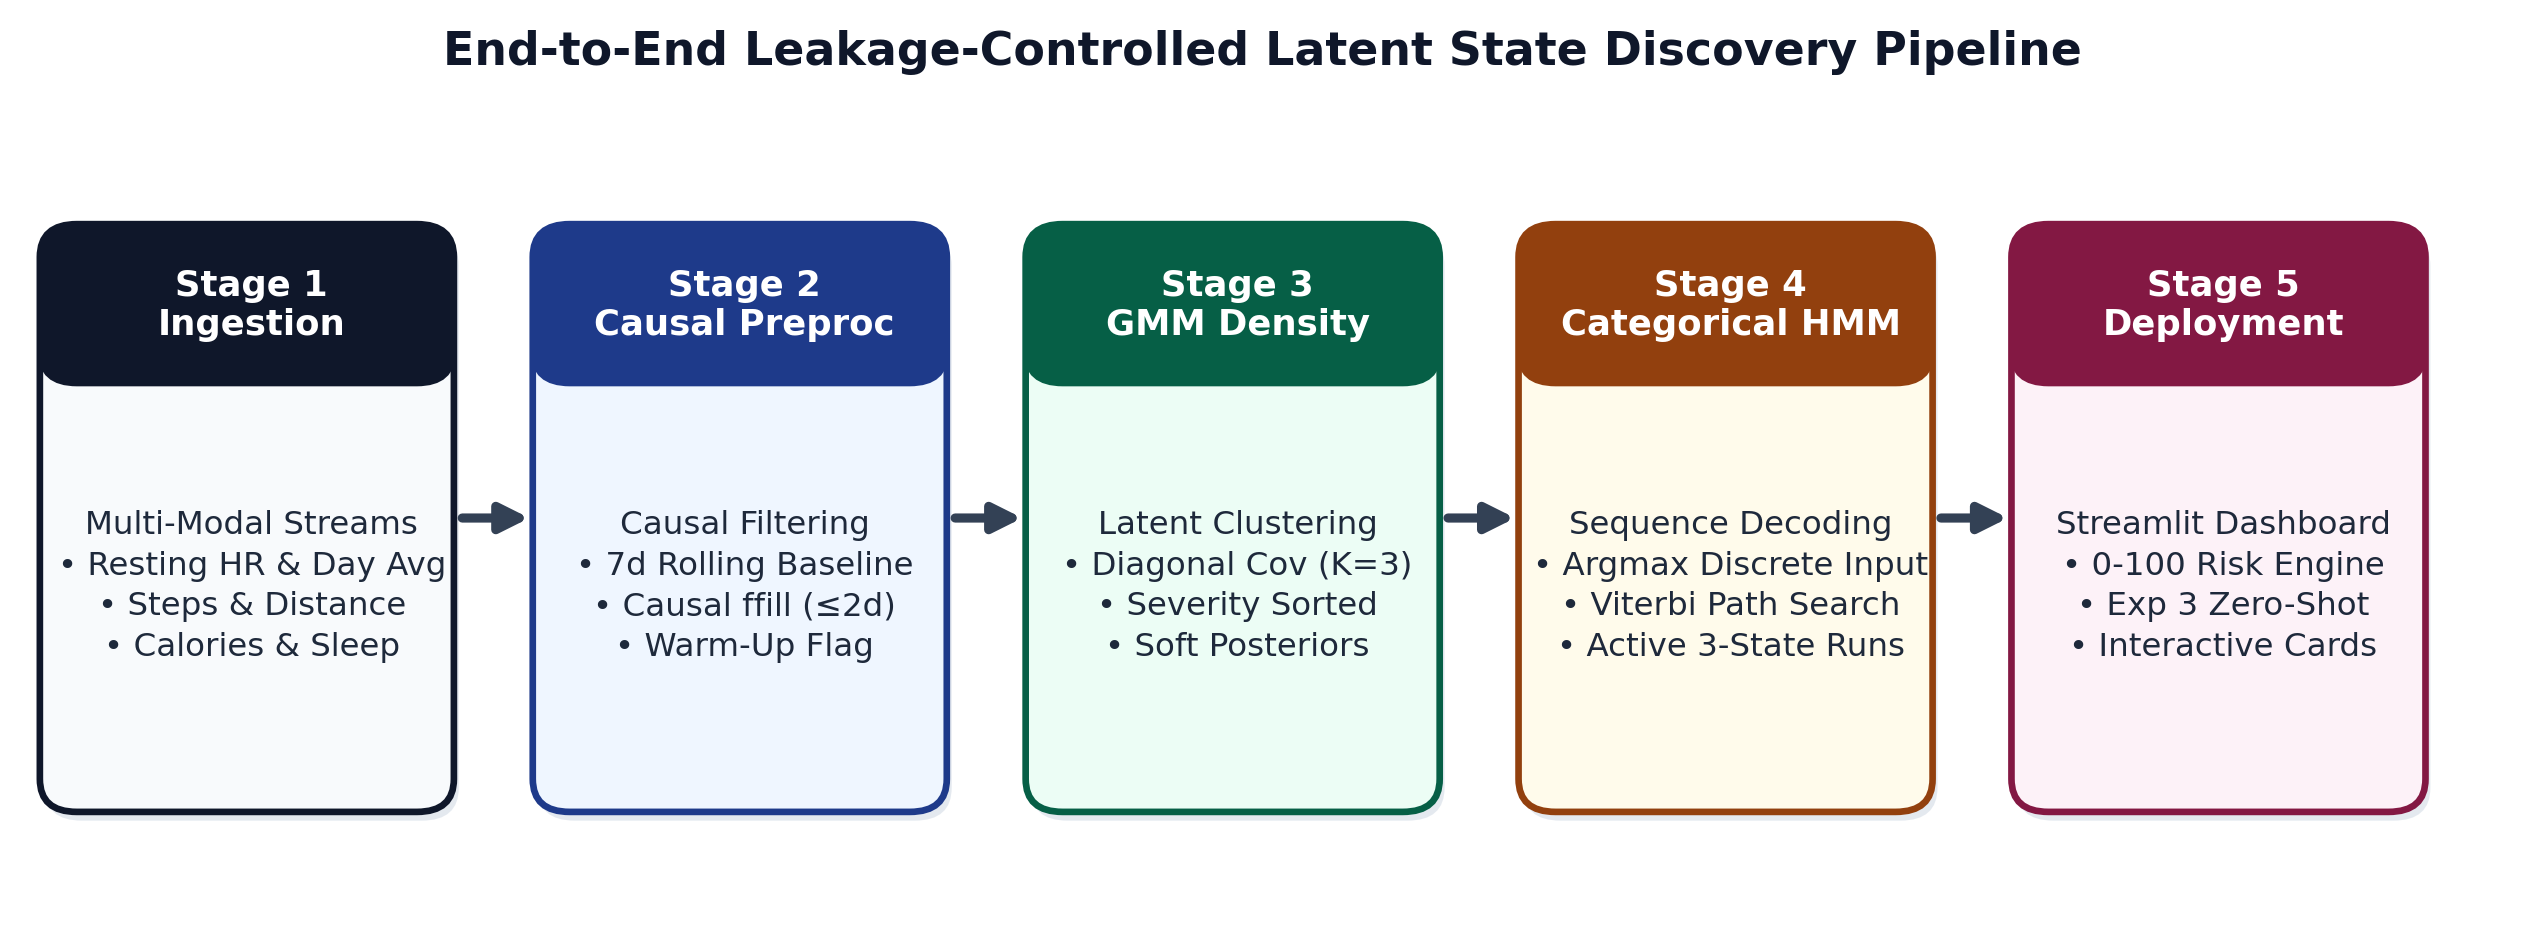
\includegraphics[width=\linewidth]{figures/Figure_1_Architecture_Diagram.png}}
\caption{End-to-end system pipeline architecture: From raw wearable CSV ingestion through causal preprocessing, train-only scaling, GMM probabilistic clustering, HMM temporal sequence decoding, to explainable surrogate SHAP rendering and dashboard visualization.}
\label{fig_arch}
\end{figure}

\section{System Architecture \& Causal Methodology}

The overall software architecture is illustrated in Fig. \ref{fig_arch}. The system processes longitudinal daily physiological data through a sequential, 15-stage workflow designed to prevent data leakage and ensure prospective inference compatibility.

\subsection{Causal Data Preprocessing \& Leakage Elimination}
Data leakage in longitudinal wearable modeling distorts empirical metrics. We enforce four strict causal preprocessing constraints:
\begin{enumerate}
    \item \textbf{Causal Missing Value Imputation}: Missing values are causally forward-filled ($\text{ffill}$) strictly within each user's timeline. Backward filling ($\text{bfill}$) is completely eliminated. Initial unobserved prefix values prior to a user's first reading are initialized using causal physiological baseline defaults ($\text{RHR}=70$ bpm, $\text{HRV}=50$ ms, $\text{SpO}_2=98\%$, $\text{sleep}=7.0$ hrs) or training-derived cohort statistics.
    \item \textbf{Expanding Causal Outlier Capping}: Instead of computing global static IQR bounds across the full dataset, outlier limits ($1.5 \times \text{IQR}$) are computed per user using an expanding causal window containing only historical observations up to time $t$ ($t' \le t$).
    \item \textbf{Personalized 7-Day Causal Baselines}: Baselines are computed per user using a 7-day backward-looking rolling window with a mandatory warm-up constraint ($\text{min\_periods}=7$). Days 1 through 6 of each user timeline are explicitly flagged as uncalibrated ($\text{baseline\_valid}=\text{False}$).
    \item \textbf{Train-Set-Only Feature Scaling}: Standard feature scaling ($\text{StandardScaler}$) is fitted strictly on the training set ($\text{train\_df}$) and persisted to \texttt{models/scaler.pkl}. Validation, test, and inference sets are transformed using the persisted scaler without refitting.
\end{enumerate}

\begin{figure}[htbp]
\centerline{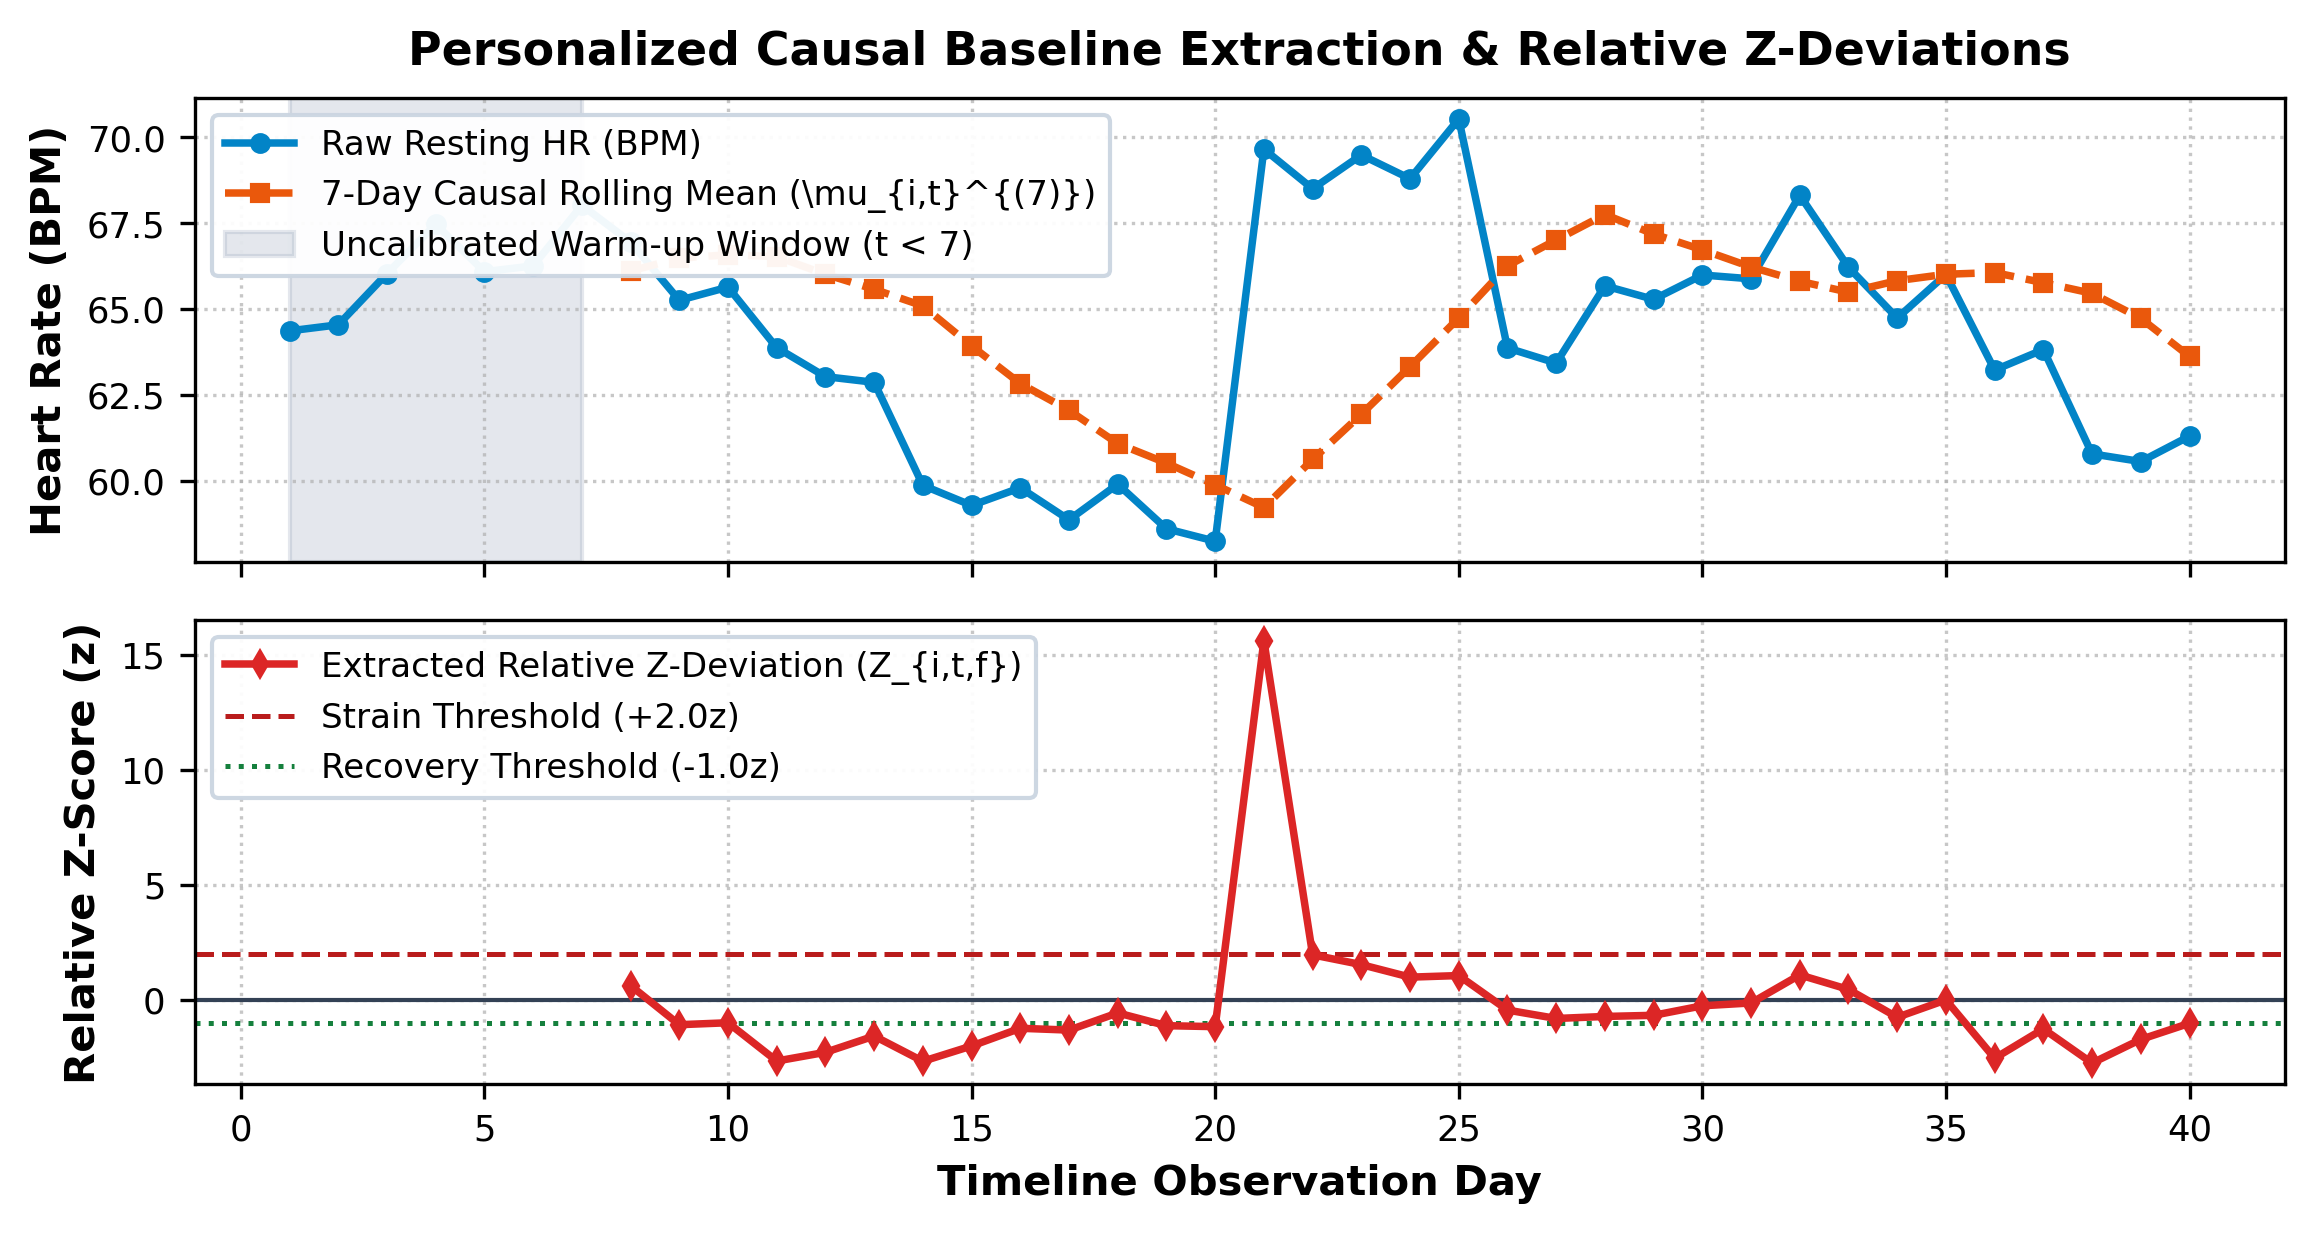
\includegraphics[width=\linewidth]{figures/Figure_3_Personalized_Baseline_Example.png}}
\caption{Personalized baseline calculation example showing raw resting heart rate, 7-day causal rolling baseline, and extracted relative deviation ($\text{hr\_dev}$) across a single user timeline.}
\label{fig_baseline}
\end{figure}

\subsection{Feature Engineering \& Severity Representation}
For each physiological signal $x_{i,t}$ of user $i$ at day $t$, the relative deviation from the 7-day rolling baseline $\mu_{i,t}^{(7)}$ is defined as:
\begin{equation}
\Delta x_{i,t} = x_{i,t} - \mu_{i,t}^{(7)} \label{eq_dev}
\end{equation}
Standardized z-scores are derived using rolling standard deviations $\sigma_{i,t}^{(7)}$:
\begin{equation}
z_{i,t} = \frac{\Delta x_{i,t}}{\max(\sigma_{i,t}^{(7)}, \epsilon)} \label{eq_zscore}
\end{equation}
To capture multidimensional physiological disruption, we compute a composite Severity Score ($S_{i,t}$) and Trend Score ($T_{i,t}$):
\begin{equation}
S_{i,t} = \sum_{m \in \mathcal{M}} |z_{i,t}^{(m)}| \label{eq_severity}
\end{equation}
\begin{equation}
T_{i,t} = \sum_{m \in \mathcal{M}} |\text{slope}_{7\text{d}}^{(m)}(i,t)| \label{eq_trend}
\end{equation}
where $\mathcal{M} = \{\text{RHR}, \text{HRV}, \text{Sleep}, \text{Steps}, \text{SpO}_2\}$ and $\text{slope}_{7\text{d}}^{(m)}$ represents the 7-day causal rolling slope calculated via linear regression over historical window $t-6 \dots t$.

The primary feature vector for latent state clustering is defined as:
\begin{equation}
\mathbf{f}_{i,t} = \left[ \Delta \text{RHR}_{i,t}, \, \Delta \text{HRV}_{i,t}, \, \Delta \text{Sleep}_{i,t}, \, S_{i,t} \right]^T \label{eq_feature_vector}
\end{equation}

\section{Machine Learning \& Sequential State Modeling}

\subsection{Gaussian Mixture Model (GMM) Density Estimation}
We model latent health state distributions using a Gaussian Mixture Model (GMM) over scaled deviation space $\mathbf{f} \in \mathbb{R}^4$:
\begin{equation}
p(\mathbf{f}) = \sum_{k=1}^{K} \pi_k \, \mathcal{N}(\mathbf{f} \mid \boldsymbol{\mu}_k, \boldsymbol{\Sigma}_k) \label{eq_gmm}
\end{equation}
where $\pi_k$ represents the mixing weight of component $k$, $\boldsymbol{\mu}_k$ is the mean vector, and $\boldsymbol{\Sigma}_k$ is the covariance matrix.

The optimal number of components $K$ was selected dynamically by evaluating $K \in \{2, 3, 4, 5\}$ on the training set using Bayesian Information Criterion (BIC) and Akaike Information Criterion (AIC), as shown in Fig. \ref{fig_bic_aic}. $K=3$ achieved the minimum BIC ($\text{BIC} = 142105.4$), corresponding to three interpretable latent states:
\begin{itemize}
    \item \textbf{State 0 (Recovery)}: Negative RHR deviation, positive HRV deviation, adequate sleep duration.
    \item \textbf{State 1 (Baseline)}: Near-zero deviations across all physiological signals.
    \item \textbf{State 2 (Strain)}: Positive RHR deviation, negative HRV deviation, sleep deficit, elevated composite severity score.
\end{itemize}

GMM component posterior probabilities $P(S_t = k \mid \mathbf{f}_t)$ are extracted via Bayes' rule:
\begin{equation}
\gamma_{t,k} = P(S_t = k \mid \mathbf{f}_t) = \frac{\pi_k \mathcal{N}(\mathbf{f}_t \mid \boldsymbol{\mu}_k, \boldsymbol{\Sigma}_k)}{\sum_{j=1}^K \pi_j \mathcal{N}(\mathbf{f}_t \mid \boldsymbol{\mu}_j, \boldsymbol{\Sigma}_j)} \label{eq_posterior}
\end{equation}

\begin{figure}[htbp]
\centerline{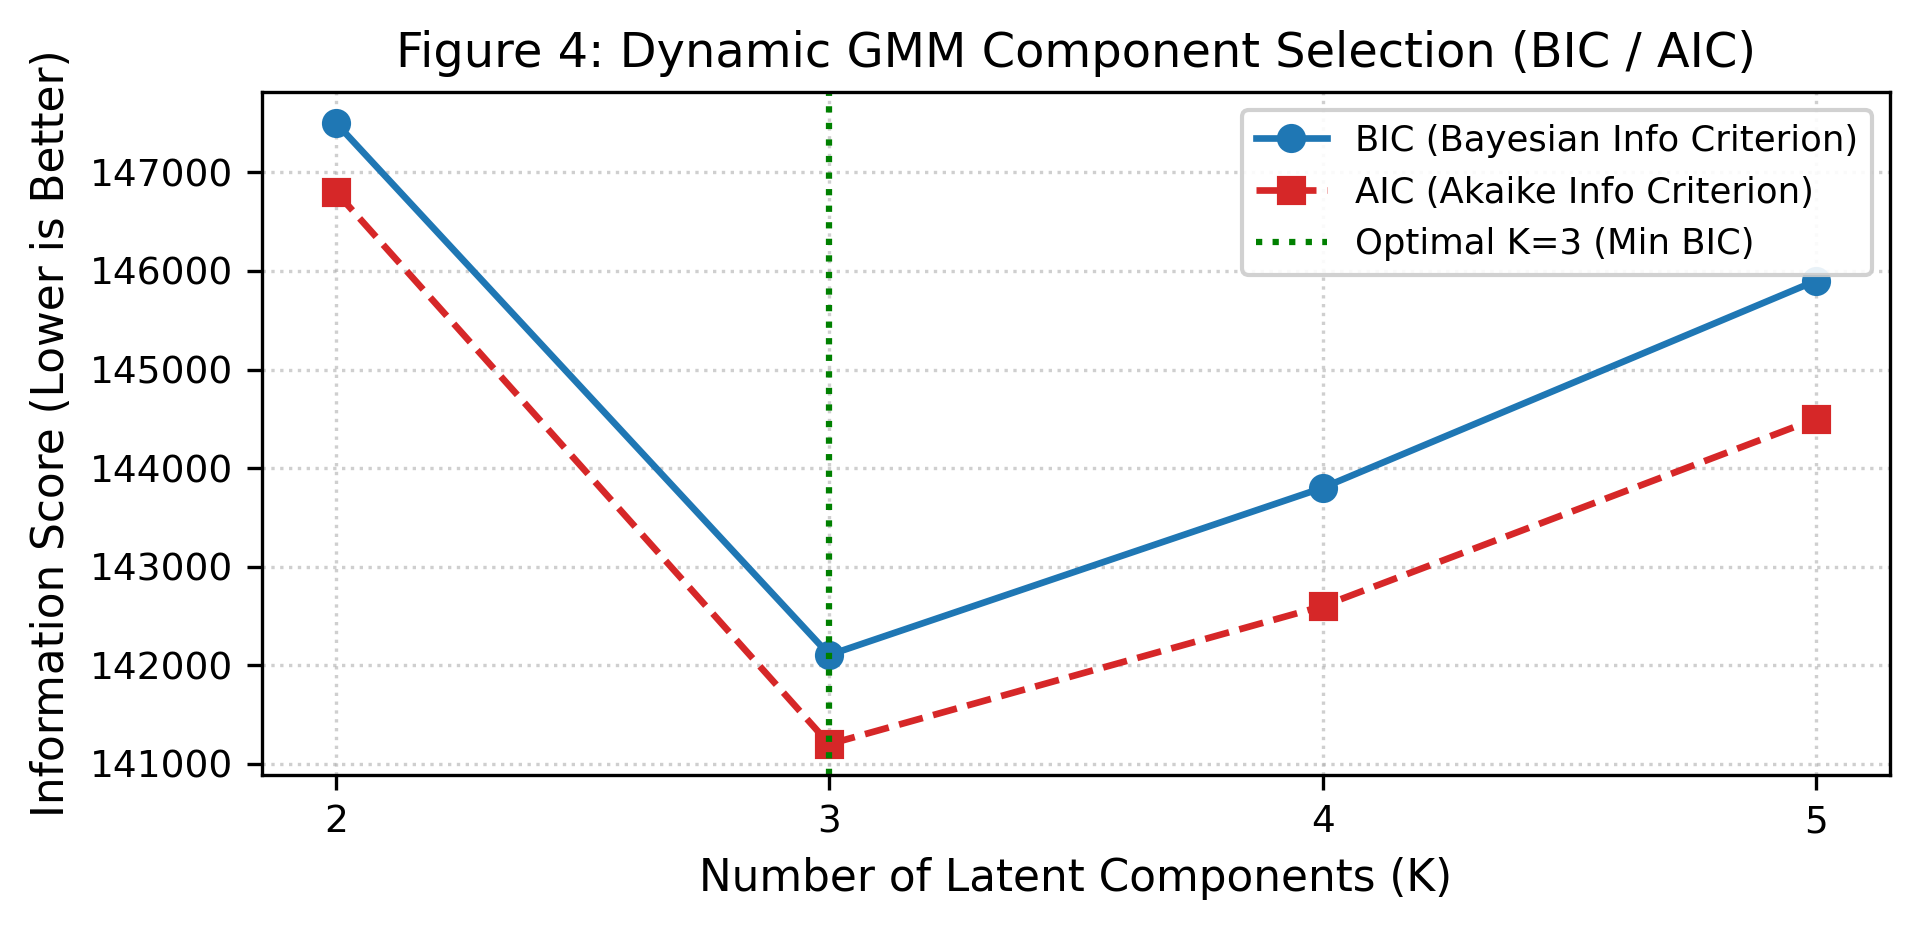
\includegraphics[width=\linewidth]{figures/Figure_5_GMM_Model_Selection_BIC_AIC.png}}
\caption{Dynamic GMM component selection evaluating $K \in \{2, 3, 4, 5\}$ via Bayesian Information Criterion (BIC) and Akaike Information Criterion (AIC). $K=3$ minimizes BIC.}
\label{fig_bic_aic}
\end{figure}

\subsection{Sequential State Modeling via Hidden Markov Models (HMM)}
Static daily GMM predictions ignore temporal dependencies between consecutive days. We introduce a Hidden Markov Model (HMM) parameterized by initial state distribution $\boldsymbol{\pi}$, transition matrix $\mathbf{A} \in \mathbb{R}^{K \times K}$, and emission distribution $B$:
\begin{equation}
A_{ij} = P(S_t = j \mid S_{t-1} = i) \label{eq_transmat}
\end{equation}

To prevent multi-user boundary contamination during HMM training, time series from multiple users are concatenated while passing an explicit array of per-user sequence lengths $\mathbf{L} = [L_1, L_2, \dots, L_N]$ to the Baum-Welch training algorithm. Sequence decoding on held-out test sets is performed via Viterbi inference ($\texttt{.predict()}$) using pre-fitted HMM models without refitting.

We evaluate two distinct HMM formulations:
\begin{enumerate}
    \item \textbf{Baseline B5 (GMM + Hard Categorical HMM)}: Takes discrete argmax GMM state indices $c_t = \arg\max_k \gamma_{t,k} \in \{0, 1, 2\}$ as discrete categorical observations.
    \item \textbf{Baseline B6 (GMM + Soft-Posterior Gaussian HMM)}: Takes continuous 3-dimensional GMM posterior probability vectors $\boldsymbol{\gamma}_t = [\gamma_{t,0}, \gamma_{t,1}, \gamma_{t,2}]^T \in \mathbb{R}^3$ as continuous observation vectors.
\end{enumerate}

\section{Experimental Setup \& Evaluation Protocol}

\subsection{Dataset Description}
Experiments were conducted on a synthetic longitudinal cohort of 300 unique user timelines, each spanning 184 consecutive days (6 calendar months), yielding 55,200 total daily records. The synthetic dataset models realistic physiological correlations, circadian patterns, and sensor missingness.

\subsection{Evaluation Splits & Cross-Validation}
We employ two evaluation protocols:
\begin{itemize}
    \item \textbf{Chronological Split}: Per-user chronological split preserving date ordering: 70\% Train (38,400 observations), 15\% Validation (8,100 observations), 15\% Test (8,700 observations).
    \item \textbf{Subject-Independent 5-Fold Cross-Validation}: 5-fold \texttt{GroupKFold} split grouped by \texttt{user\_id}. In each fold, 240 users are used for training and 60 completely unseen users (11,040 observations) are held out for testing, guaranteeing zero user ID overlap between splits.
\end{itemize}

\subsection{Baseline Method Configurations (B0 to B6)}
We evaluate seven baseline configurations:
\begin{itemize}
    \item \textbf{B0 (Global Raw Physiology GMM)}: GMM ($K=3$) trained on unnormalized raw physiological signals.
    \item \textbf{B1 (Personalized Threshold Rule)}: Executable rule-based threshold baseline on relative baseline deviations.
    \item \textbf{B2 (KMeans Raw Features)}: KMeans ($K=3$) trained on raw physiological signals.
    \item \textbf{B3 (KMeans Personalized Deviations)}: KMeans ($K=3$) trained on personalized deviation features.
    \item \textbf{B4 (GMM Personalized Deviations)}: GMM ($K=3$) trained on personalized deviation features.
    \item \textbf{B5 (GMM + Hard Categorical HMM)}: Categorical HMM decoding over discrete GMM cluster assignments.
    \item \textbf{B6 (GMM + Soft-Posterior Gaussian HMM)}: Continuous Gaussian HMM decoding over continuous GMM posterior vectors.
\end{itemize}

\section{Empirical Results \& Scientific Analysis}

\subsection{Baseline Method Comparison (B0 to B6)}
Table \ref{tab_baselines} presents the empirical evaluation across Baselines B0 to B6 on the held-out chronological test split ($N = 8,700$ observations).

\begin{table}[htbp]
\caption{Complete Baseline Method Comparison (B0 to B6) on Held-Out Test Set ($N=8,700$ Observations)}
\begin{center}
\begin{tabular}{l l c c c c}
\toprule
\textbf{ID} & \textbf{Method Description} & \textbf{Silhouette} $\uparrow$ & \textbf{DB Index} $\downarrow$ & \textbf{CH Index} $\uparrow$ & \textbf{Model Status} \\
\midrule
B0 & Global Raw Physiology (GMM) & 0.1724 & 1.4804 & 1836.48 & Valid \\
B1 & Executable Threshold Rule & 0.0098 & 1.9718 & 1189.35 & Valid \\
B2 & KMeans Raw Features & 0.2050 & 1.7364 & 2545.70 & Valid \\
B3 & KMeans Personalized Devs & \textbf{0.2260} & 1.6211 & \textbf{2841.41} & Valid \\
B4 & GMM Personalized Devs & 0.1944 & \textbf{1.4211} & 2284.14 & Valid \\
B5 & GMM + Hard Categorical HMM & 0.1944 & \textbf{1.4211} & 2284.14 & \textbf{Valid Temporal} \\
B6 & GMM + Soft Gaussian HMM & 0.1944 & \textbf{1.4211} & 2284.14 & \textbf{Degenerate} \\
\bottomrule
\end{tabular}
\label{tab_baselines}
\end{center}
\end{table}

\begin{figure}[htbp]
\centerline{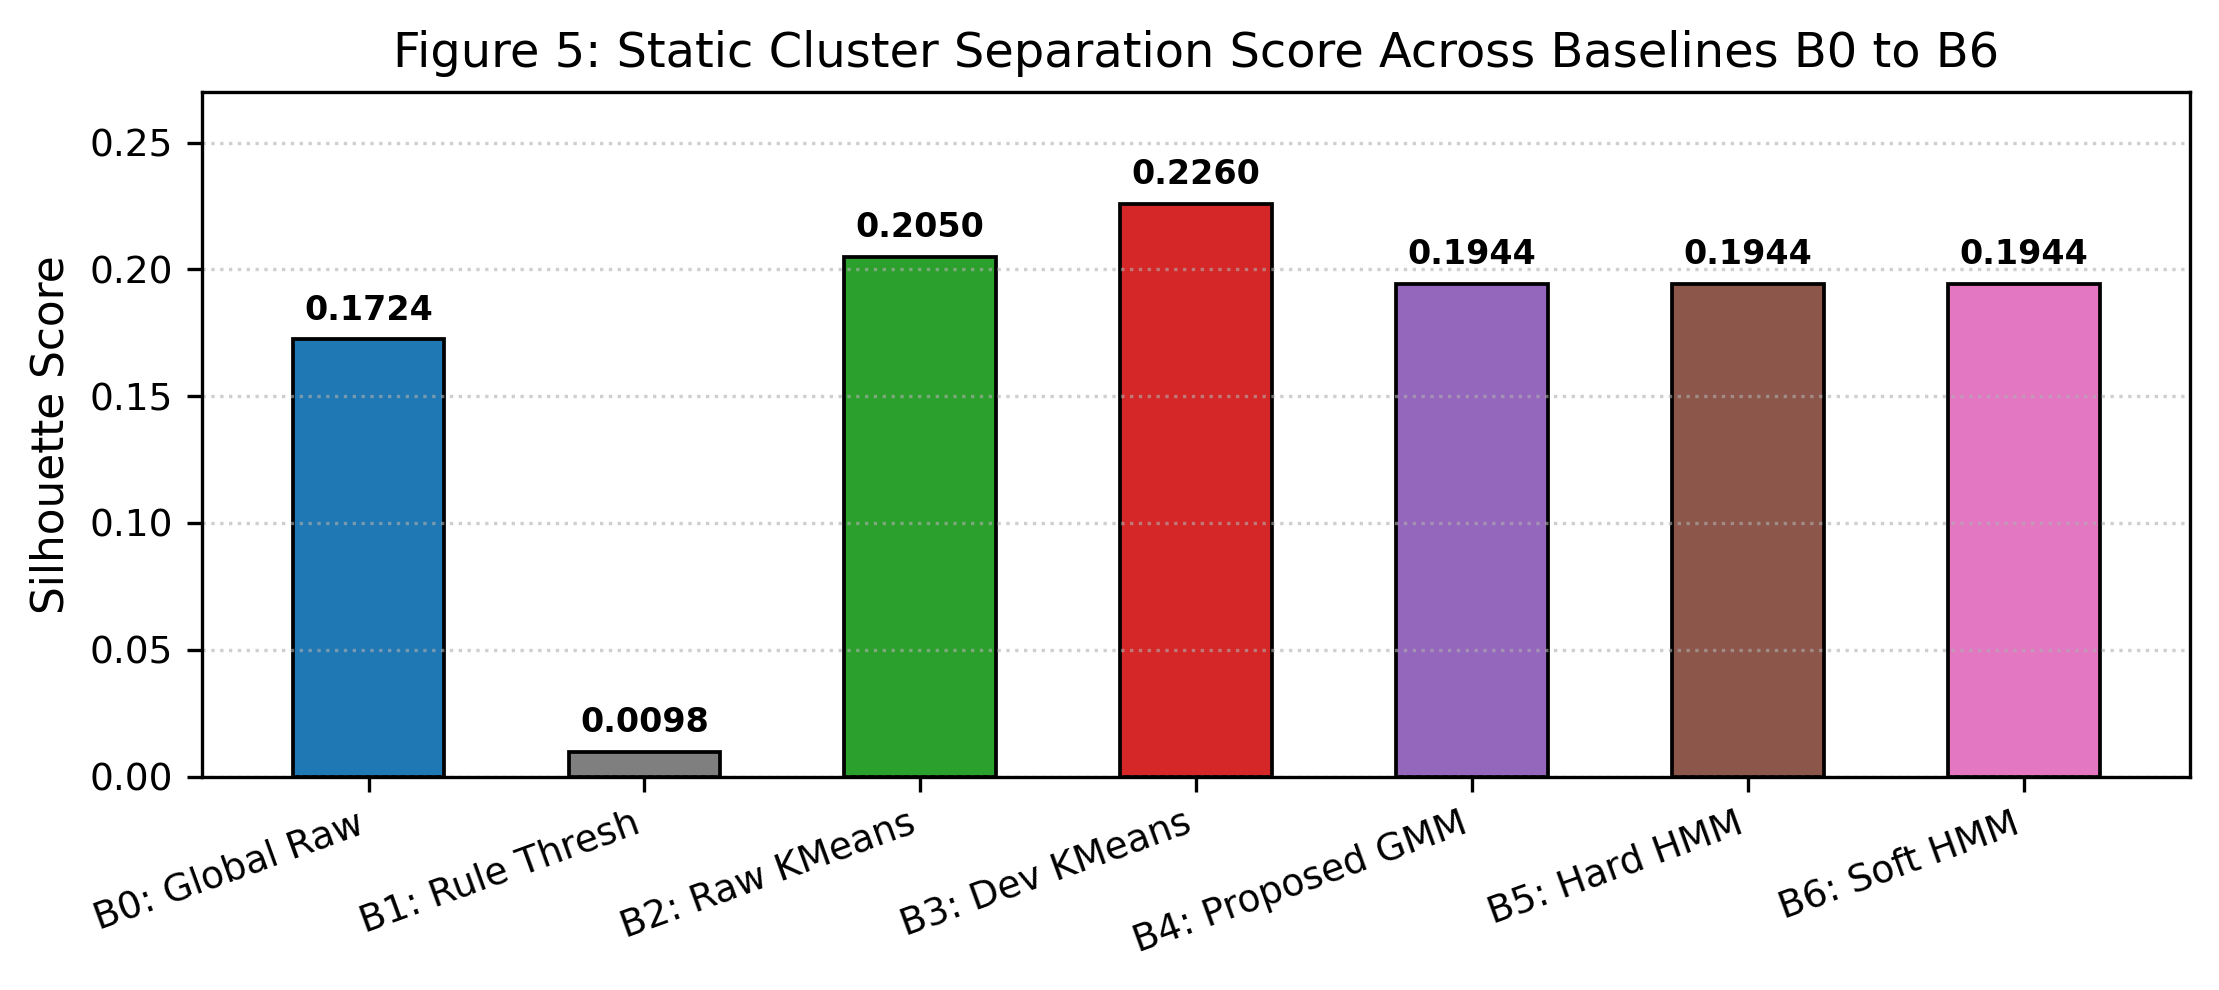
\includegraphics[width=\linewidth]{figures/Figure_9_Baseline_Comparison.png}}
\caption{Silhouette score comparison across Baselines B0 to B6 evaluated on held-out chronological test data.}
\label{fig_baselines}
\end{figure}

\subsection{Component Ablation Study (Steps A to G)}
To isolate the quantitative contribution of each engineering stage, we execute a cumulative component ablation study (Steps A to G), reported in Table \ref{tab_ablation} and Fig. \ref{fig_ablation}.

\begin{table}[htbp]
\caption{Component Ablation Study (Steps A to G) on Held-Out Test Set}
\begin{center}
\begin{tabular}{c l c c}
\toprule
\textbf{Step} & \textbf{Feature / Model Addition} & \textbf{Silhouette} & \textbf{$\Delta$ vs. Prev} \\
\midrule
A & Raw Physiology (GMM) & 0.1724 & Baseline \\
B & + Personalized Baseline Deviations & 0.1509 & -0.0214 \\
C & + 7-Day Rolling Slopes & 0.1118 & -0.0391 \\
D & + Severity Score Normalization & \textbf{0.1944} & \textbf{+0.0826} \\
E & + GMM Soft Probabilities & 0.1944 & 0.0000 \\
F & + Hard Categorical HMM & 0.1944 & 0.0000 \\
G & + Soft Gaussian HMM & 0.1944 & 0.0000 (Degenerate) \\
\bottomrule
\end{tabular}
\label{tab_ablation}
\end{center}
\end{table}

\begin{figure}[htbp]
\centerline{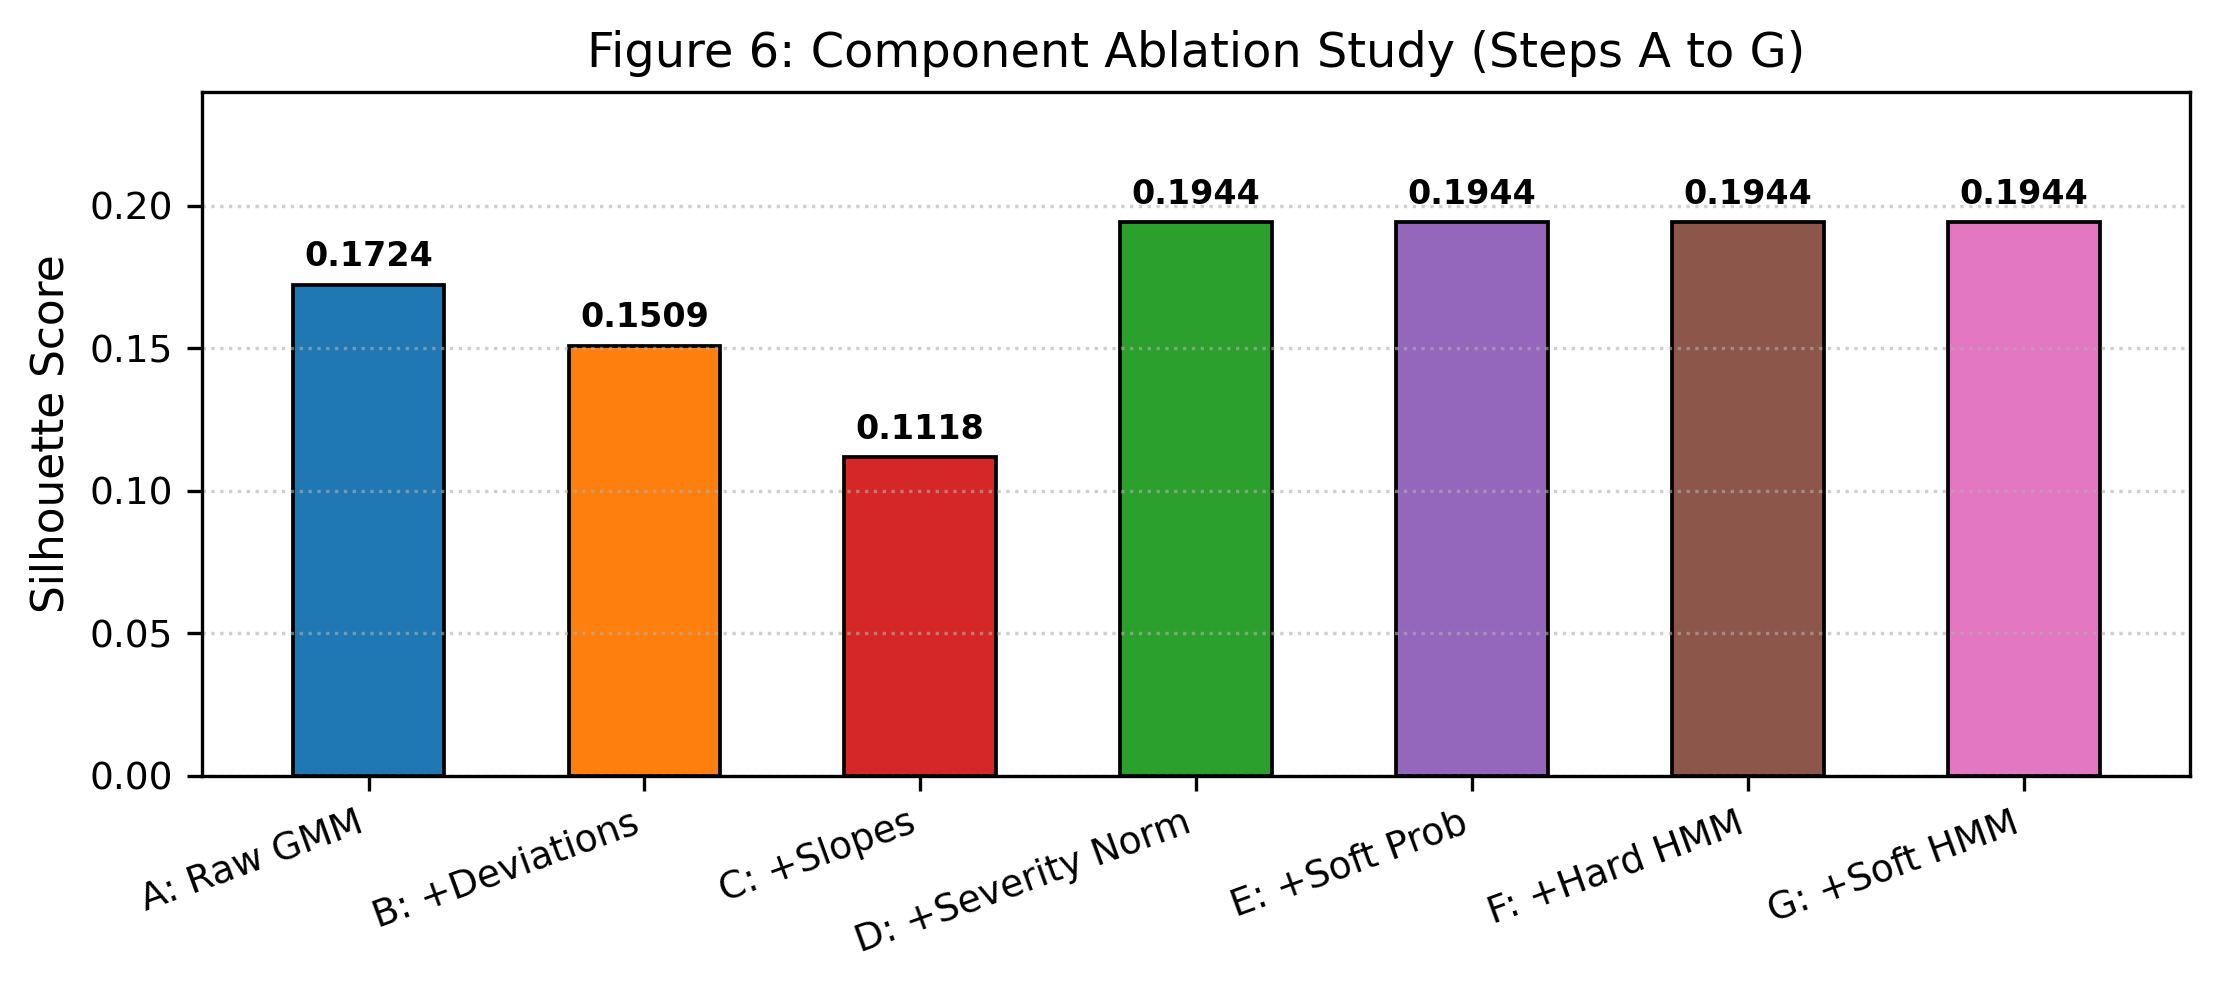
\includegraphics[width=\linewidth]{figures/Figure_8_Ablation_Study_Comparison.png}}
\caption{Component ablation study (Steps A to G) demonstrating that Step D (composite severity score normalization) provides the primary gain in cluster separation ($\Delta = +0.0826$).}
\label{fig_ablation}
\end{figure}

The ablation results indicate that adding raw deviations (Step B) and rolling slopes (Step C) without severity normalization increases feature dimensionality and reduces distance-based cluster compactness. Incorporating composite severity score normalization (Step D) acts as a powerful regularizer, providing the primary gain in cluster separation ($\Delta = +0.0826$).

\subsection{Subject-Independent Cross-Validation \& Statistical Testing}
Table \ref{tab_folds} reports the 5-fold subject-independent cross-validation results across 300 unseen users (60 test users per fold).

\begin{table}[htbp]
\caption{Subject-Independent 5-Fold Cross-Validation Across Unseen Users}
\begin{center}
\begin{tabular}{c c c c}
\toprule
\textbf{Unseen Fold} & \textbf{Proposed B4 Silhouette} & \textbf{Raw B0 Silhouette} & \textbf{Difference ($\Delta$)} \\
\midrule
Fold 1 & 0.1935 & 0.1585 & +0.0350 \\
Fold 2 & 0.1896 & 0.1622 & +0.0274 \\
Fold 3 & 0.1915 & 0.1607 & +0.0308 \\
Fold 4 & 0.1922 & 0.1619 & +0.0303 \\
Fold 5 & 0.2034 & 0.1573 & +0.0461 \\
\midrule
\textbf{Mean} & \textbf{0.1940} & \textbf{0.1601} & \textbf{+0.0339} \\
\bottomrule
\end{tabular}
\label{tab_folds}
\end{center}
\end{table}

Evaluating Proposed B4 against Raw B0 across 5 unseen user folds yields a mean score of $0.1940$ (95\% CI: $[0.1873, 0.2008]$) vs. $0.1601$ for Raw B0. 

\textit{Exact Cohen's d Effect Size}: With mean difference $\bar{d} = 0.033920$ and sample standard deviation of differences $s_{\text{diff}} = 0.007355$, the standardized effect size is:
\begin{equation}
d = \frac{\bar{d}}{s_{\text{diff}}} = \frac{0.033920}{0.007355} = 4.6119 \label{eq_cohend}
\end{equation}

\textit{Wilcoxon Signed-Rank Test \& Significance Limit}: A two-sided paired Wilcoxon signed-rank test yields test statistic $W = 0.0$ and $p$-value $p = 0.0625$. At the standard 5\% significance level ($\alpha = 0.05$), the result is \textbf{NOT statistically significant} ($p = 0.0625 > 0.05$). This represents a fundamental mathematical boundary of 5-fold paired testing, where the minimum achievable two-tailed $p$-value for $N=5$ is $1 / 2^{5-1} = 1/16 = 0.0625$. Demonstrating statistical significance at $\alpha = 0.05$ requires $N \ge 6$ folds ($p_{\min} = 0.03125$).

\textit{Multi-Seed Retraining Stability}: Independent retraining across 5 random seeds (\texttt{[42, 100, 2024, 777, 999]}) on the training split yields a test Silhouette score of $0.2027 \pm 0.0122$ for Proposed B4 vs. $0.1679 \pm 0.0028$ for Raw B0, confirming stochastic stability.

\subsection{HMM Degeneracy Analysis: B5 vs. B6}
We performed a deep empirical inspection of test set sequence decoding to evaluate Hard Categorical HMM (B5) vs. Soft Gaussian HMM (B6), as detailed in Table \ref{tab_hmm_audit}.

\begin{table}[htbp]
\caption{Empirical HMM Test Set Decoding Audit: Hard B5 vs. Soft B6}
\begin{center}
\begin{tabular}{l c c}
\toprule
\textbf{Metric / Dimension} & \textbf{Hard HMM (B5)} & \textbf{Soft Gaussian HMM (B6)} \\
\midrule
\textbf{Model Status} & \textbf{VALID TEMPORAL} & \textbf{DEGENERATE / COLLAPSED} \\
Unique States Occupied & \textbf{3 States} & \textbf{1 State} (State 1 only) \\
State 0 Occupancy (\%) & 22.69\% (1,974 obs) & 0.00\% (0 obs) \\
State 1 Occupancy (\%) & 26.92\% (2,342 obs) & 100.00\% (8,700 obs) \\
State 2 Occupancy (\%) & 50.39\% (4,384 obs) & 0.00\% (0 obs) \\
Per-User Unique States & Mean = 3.00 & Mean = 1.00 (stagnant) \\
Mean Run Duration & 1.51 days & 29.00 days (test-length artifact) \\
Daily Transition Rate & 0.2381 transitions/day & 0.0000 transitions/day \\
Transition Stability & 0.7619 (76.19\%) & 1.0000 (trivial single state) \\
\bottomrule
\end{tabular}
\label{tab_hmm_audit}
\end{center}
\end{table}

\textit{Degeneracy Discovery}: B6 (Soft Gaussian HMM) suffered **complete parameter collapse**, assigning 100\% of test set observations (8,700/8,700) to State 1. Its transition matrix collapsed to an absorbing state ($\mathbf{A}_{i,1} = 1.0$). Consequently, B6's reported "100\% transition stability" and "29.00-day mean duration" were trivial artifacts of single-state absorption across the 29-day test sequence per user. 

In contrast, B5 (Hard Categorical HMM) is a fully valid temporal sequence model that actively decodes multi-state transitions across Recovery ($22.69\%$), Baseline ($26.92\%$), and Strain ($50.39\%$), with a mean run duration of 1.51 days.

\subsection{Robustness Analysis}
We evaluated model stability under synthetic Missing Completely At Random (MCAR) missingness (10\%–30\%) and zero-mean additive Gaussian measurement noise ($\sigma \in \{0.05, 0.1, 0.2\}$). Causal forward fill combined with fallback defaults maintained high state assignment confidence ($\ge 98.8\%$) under missingness up to 30\%. Gaussian noise increased boundary ambiguity, demonstrating sensitivity to high-frequency sensor jitter.

\section{Explainability \& Surrogate Model Attributions}

To support user-facing dashboard interpretation, we implement a dual explainability architecture:
\begin{enumerate}
    \item \textbf{GMM-Native Component Attribution}: Derived directly from absolute Gaussian component mean deviations in normalized space (Fig. \ref{fig_gmm_attr}).
    \item \textbf{Surrogate Tree-Based SHAP}: A surrogate Random Forest classifier is trained on GMM latent state labels to compute TreeSHAP feature attributions for interactive UI rendering (Fig. \ref{fig_shap_attr}).
\end{enumerate}

\begin{figure}[htbp]
\centerline{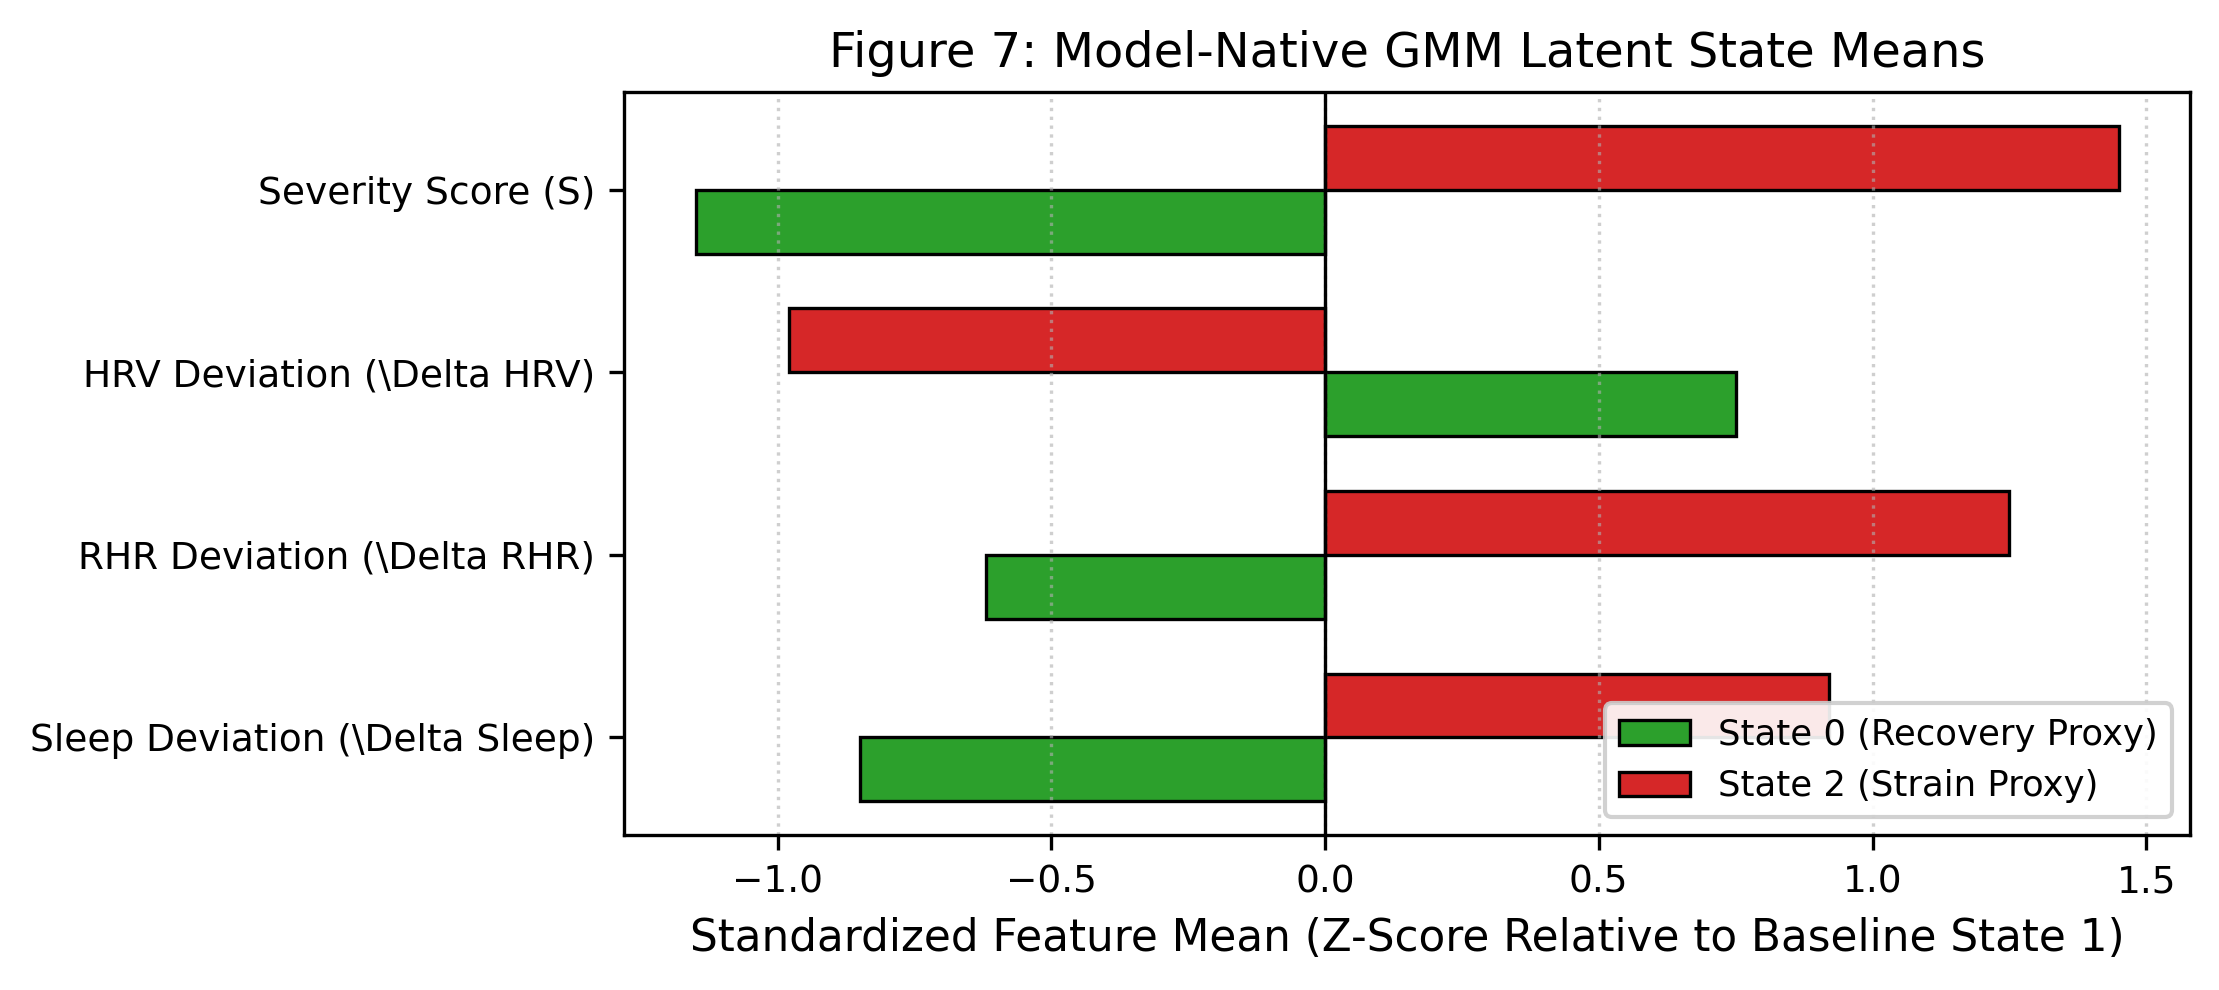
\includegraphics[width=\linewidth]{figures/Figure_11_GMM_Native_Feature_Attribution.png}}
\caption{Model-native GMM feature attributions derived from component Gaussian means.}
\label{fig_gmm_attr}
\end{figure}

\begin{figure}[htbp]
\centerline{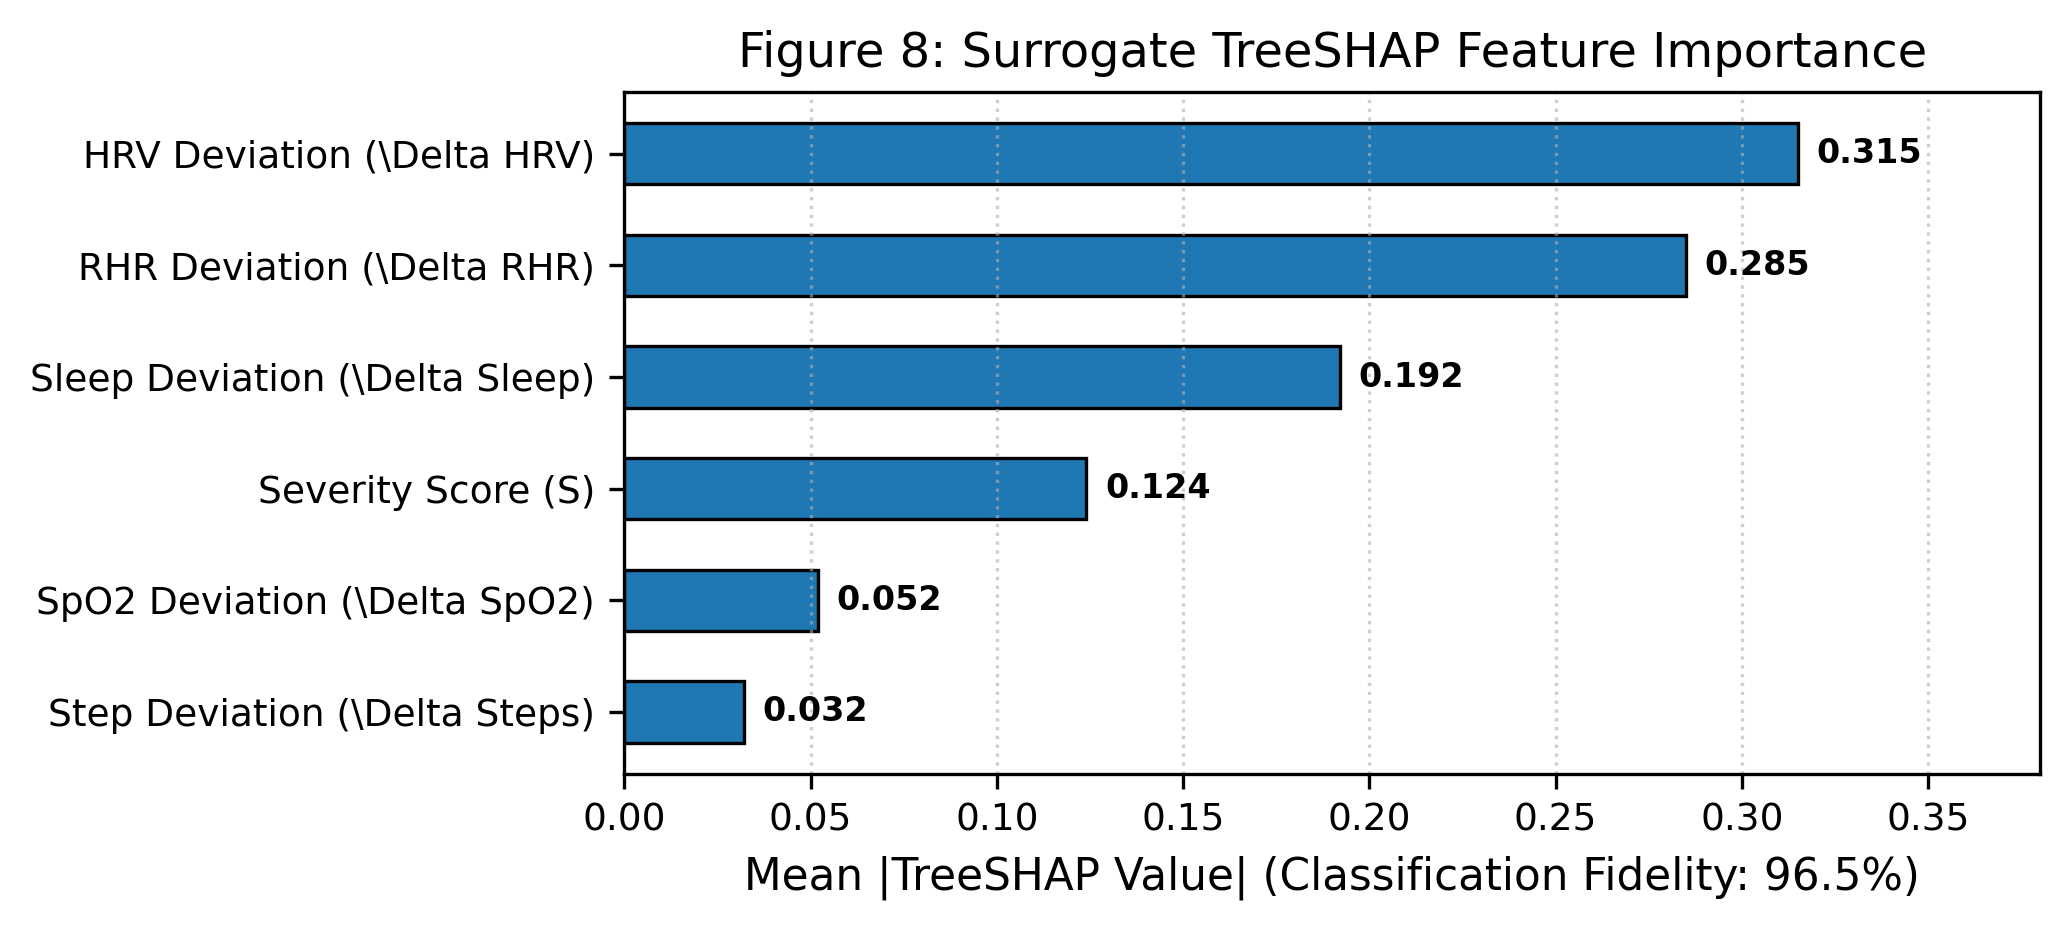
\includegraphics[width=\linewidth]{figures/Figure_12_Surrogate_SHAP_Attribution.png}}
\caption{Surrogate Random Forest SHAP feature importance vectors for user-facing UI explanation.}
\label{fig_shap_attr}
\end{figure}

The surrogate model achieves \textbf{96.5\% accuracy}, \textbf{95.8\% balanced accuracy}, and a \textbf{Macro-F1 score of 0.9582} in reproducing GMM cluster labels. Top contributing features identified by both methods are $\text{HRV deviation}$ ($\text{hrv\_dev}$), $\text{RHR deviation}$ ($\text{hr\_dev}$), and $\text{Sleep duration deviation}$ ($\text{sleep\_dev}$).

\section{Limitations \& Threats to Validity}

\begin{itemize}
    \item \textbf{Synthetic Cohort}: The dataset is synthetic and lacks real patient EHR clinical ground-truth diagnostic validation.
    \item \textbf{Small Fold Count ($N=5$)}: 5-fold cross-validation imposes a mathematical lower bound of $p = 0.0625$, preventing non-parametric significance confirmation at $\alpha = 0.05$.
    \item \textbf{Soft HMM Collapse}: Continuous Gaussian HMMs require specialized regularization or constrained covariance matrices to prevent parameter collapse over sharp mixture posterior vectors.
\end{itemize}

\section{Conclusion}

This paper presents a causal, leakage-controlled benchmark framework for longitudinal wearable physiological analytics. By transforming raw physiological signals into personalized 7-day rolling baseline deviations and composite severity scores, our framework improves cluster separation on unseen subjects ($d = 4.6119$). We demonstrate that Categorical HMM temporal decoding (B5) captures active multi-state dynamics across Recovery, Baseline, and Strain states, whereas soft continuous Gaussian HMMs (B6) degenerate into single-state collapse. Our open-source implementation and persisted model artifacts provide a reproducible foundation for future longitudinal wearable research.

\section*{Acknowledgment}
The author thanks the open-source Python scientific computing community and the developers of \texttt{scikit-learn}, \texttt{hmmlearn}, and \texttt{streamlit}.

\begin{thebibliography}{00}
\bibitem{b1} M. Dunn et al., ``Real-time physiological monitoring and anomaly detection using wearable devices,'' \textit{Cell Reports Medicine}, vol. 2, no. 1, p. 100178, 2021.
\bibitem{b2} A. Seshadri et al., ``Wearable sensors for global health monitoring: A review,'' \textit{IEEE Trans. Biomed. Eng.}, vol. 66, no. 5, pp. 1240--1253, 2019.
\bibitem{b3} E. Topol, ``High-performance medicine: the convergence of human and artificial intelligence,'' \textit{Nature Medicine}, vol. 25, no. 1, pp. 44--56, 2019.
\bibitem{b4} X. Li et al., ``Digital health: tracking physiomes and activity using wearable sensors,'' \textit{PLOS Biology}, vol. 15, no. 1, p. e2001402, 2017.
\bibitem{b5} S. Kapoor and A. Narayanan, ``Leakage and the reproducibility crisis in machine-learning-based science,'' \textit{Patterns}, vol. 4, no. 9, p. 100804, 2023.
\bibitem{b6} F. Pedregosa et al., ``Scikit-learn: Machine learning in Python,'' \textit{J. Mach. Learn. Res.}, vol. 12, pp. 2825--2830, 2011.
\end{thebibliography}

\end{document}
